% !TEX program = pdflatex
\documentclass[10pt]{article}

\usepackage[utf8]{inputenc}
\usepackage[T1]{fontenc}
\usepackage[english]{babel}
\usepackage{lmodern}
\usepackage{microtype}
\usepackage[margin=0.72in]{geometry}
\usepackage{amsmath,amssymb,amsthm,mathtools}
\usepackage{booktabs,array}
\usepackage{graphicx}
\usepackage{xcolor}
\usepackage{enumitem}
\usepackage[most]{tcolorbox}
\usepackage{fancyhdr}
\usepackage[hidelinks]{hyperref}

\definecolor{CourseBlue}{HTML}{1A3C68}
\definecolor{CourseGreen}{HTML}{216E39}
\definecolor{CourseGold}{HTML}{B8860B}
\definecolor{CourseRed}{HTML}{9A2C2C}
\definecolor{SoftBlue}{HTML}{F2F6FA}
\definecolor{SoftGreen}{HTML}{F1F8F3}
\definecolor{SoftGold}{HTML}{FFF8E8}
\definecolor{SoftRed}{HTML}{FFF3F3}

\setlength{\parindent}{0pt}
\setlength{\parskip}{0.32em}
\setlist[itemize]{leftmargin=1.5em,itemsep=0.12em,topsep=0.2em}
\setlist[enumerate]{leftmargin=1.7em,itemsep=0.12em,topsep=0.2em}
\allowdisplaybreaks

\pagestyle{fancy}
\fancyhf{}
\lhead{Stochastic Calculus and Option Pricing}
\rhead{Lecture 9 Notes}
\cfoot{\thepage}
\renewcommand{\headrulewidth}{0.3pt}

\newcommand{\E}{\mathbb E}
\newcommand{\Pp}{\mathbb P}
\newcommand{\Q}{\mathbb Q}
\newcommand{\R}{\mathbb R}
\newcommand{\1}{\mathbf 1}
\newcommand{\cF}{\mathcal F}
\newcommand{\dd}{\,\mathrm d}
\newcommand{\Ncdf}{\Phi}

\theoremstyle{definition}
\newtheorem{definition}{Definition}[section]
\newtheorem{proposition}[definition]{Proposition}
\newtheorem{theorem}[definition]{Theorem}
\newtheorem{lemma}[definition]{Lemma}
\newtheorem{corollary}[definition]{Corollary}
\newtheorem{remark}[definition]{Remark}

\newtcolorbox{boardexample}[1]{
  enhanced,breakable,colback=SoftBlue,colframe=CourseBlue,
  boxrule=0.55pt,arc=1mm,left=1.5mm,right=1.5mm,top=1mm,bottom=1mm,
  before skip=0.55em,after skip=0.55em,
  title={Example --- #1},fonttitle=\bfseries}
\newtcolorbox{studentexercise}[1]{
  enhanced,breakable,colback=SoftGold,colframe=CourseGold,
  boxrule=0.55pt,arc=1mm,left=1.5mm,right=1.5mm,top=1mm,bottom=1mm,
  before skip=0.55em,after skip=0.35em,
  title={Exercise --- #1},fonttitle=\bfseries}
\newtcolorbox{shortsolution}[1][] {
  enhanced,breakable,colback=SoftGreen,colframe=CourseGreen,
  boxrule=0.55pt,arc=1mm,left=1.5mm,right=1.5mm,top=1mm,bottom=1mm,
  before skip=0.25em,after skip=0.6em,
  title={Short solution#1},fonttitle=\bfseries}
\newtcolorbox{keyidea}[1]{
  enhanced,breakable,colback=white,colframe=CourseGreen,
  boxrule=0.7pt,arc=1mm,left=1.5mm,right=1.5mm,top=1mm,bottom=1mm,
  before skip=0.5em,after skip=0.5em,
  title={#1},fonttitle=\bfseries}
\newtcolorbox{warningbox}[1]{
  enhanced,breakable,colback=SoftRed,colframe=CourseRed,
  boxrule=0.65pt,arc=1mm,left=1.5mm,right=1mm,top=1mm,bottom=1mm,
  before skip=0.5em,after skip=0.5em,
  title={#1},fonttitle=\bfseries}
\newtcolorbox{assumptionbox}[1]{
  enhanced,breakable,colback=SoftGold,colframe=CourseGold,
  boxrule=0.65pt,arc=1mm,left=1.5mm,right=1.5mm,top=1mm,bottom=1mm,
  before skip=0.5em,after skip=0.5em,
  title={#1},fonttitle=\bfseries}

\title{\textbf{Vanilla Options in Practice}\\
\large Lecture 9 Notes --- Payoffs, Black--Scholes Benchmarks, and Static-Arbitrage Diagnostics}
\author{}
\date{}

\begin{document}
\maketitle
\vspace{-1.4em}

\begin{keyidea}{Goals and logical structure}
Lecture~8 developed model-free no-arbitrage principles. This lecture applies
them to the option quotes observed in a market:
\[
\begin{aligned}
\text{option payoffs}
&\longrightarrow \text{replication and put--call parity}\\
&\longrightarrow \text{Black--Scholes benchmark prices}\\
&\longrightarrow \text{model-free bounds and strike-shape checks}\\
&\longrightarrow \text{explicit arbitrage trades.}
\end{aligned}
\]
The recurring method is always the same: write the terminal payoff of a
portfolio, compare it state by state, then translate the comparison into a
price inequality or a trading strategy.
\end{keyidea}

% ============================================================
\section{Payoffs and market language}
% ============================================================

\subsection{European calls and puts}

\begin{definition}[European vanilla options]
Let \(S_T\) be the price of an underlying asset at maturity \(T\), and let
\(K\) be a strike price. A European call gives its holder the right to buy one
share for \(K\) at \(T\); a European put gives its holder the right to sell
one share for \(K\) at \(T\). Their terminal payoffs are
\[
\boxed{(S_T-K)^+}\qquad\text{and}\qquad\boxed{(K-S_T)^+},
\]
respectively. European means that exercise is possible only at \(T\).
\end{definition}

The option holder chooses whether to exercise. For a call, paying \(K\) to
receive a share is useful only when \(S_T>K\); for a put, selling a share for
\(K\) is useful only when \(S_T<K\). A short position has the negative of the
corresponding payoff.

\begin{boardexample}{reading a payoff table}
For \(K=100\),
\[
\begin{array}{c|ccc}
S_T &80&100&130\\ \hline
(S_T-100)^+&0&0&30\\
(100-S_T)^+&20&0&0
\end{array}
\]
The call is upside exposure. The put is downside insurance.
\end{boardexample}

\subsection{Moneyness and time value}

Moneyness compares the current spot price \(S_t\) with the strike \(K\):
\[
\begin{array}{c|ccc}
&\text{in the money}&\text{at the money}&\text{out of the money}\\ \hline
\text{call}&S_t>K&S_t\approx K&S_t<K\\
\text{put}&S_t<K&S_t\approx K&S_t>K.
\end{array}
\]
It is a statement about immediate exercise value, not a forecast of whether
the option will finish in the money at \(T\).

For a call, the intrinsic value is \((S_t-K)^+\); for a put it is
\((K-S_t)^+\). The remaining part of the market price is its \emph{time
value}. At-the-money options often have the greatest time value because their
intrinsic value is near zero while there is still substantial scope for a
favourable move.

\begin{studentexercise}{which contract is mostly time value?}
Three calls have the same maturity and current spot \(S_t=100\), but strikes
\(80\), \(100\), and \(130\). Which call is most naturally interpreted as
mostly time value?
\end{studentexercise}
\begin{shortsolution}
The call struck at \(100\) is at the money, so its intrinsic value is zero.
Its price is principally the value of the uncertainty that remains before
maturity. The \(K=80\) call already has intrinsic value; the \(K=130\) call
is far out of the money and generally has a small premium.
\end{shortsolution}

\subsection{Useful payoff combinations}

Payoff algebra is often the quickest way to identify a trading strategy.
\[
\begin{aligned}
\text{long straddle:}\quad &(S_T-K)^+ +(K-S_T)^+=|S_T-K|,\\
\text{protective put:}\quad&S_T+(K-S_T)^+=\max(S_T,K),\\
\text{covered call:}\quad&S_T-(S_T-K)^+=\min(S_T,K).
\end{aligned}
\]
Thus a straddle benefits from a large move in either direction; a protective
put retains stock upside while imposing a floor \(K\); a covered call caps
stock upside at \(K\).

% ============================================================
\section{Put--call parity}
% ============================================================

\subsection{Replication identity}

Let \(D_t=e^{-r(T-t)}\) denote the price at time \(t\) of one dollar paid at
time \(T\), for a constant rate \(r\). Consider a call and a put on the same
stock, with the same \(K\) and \(T\), and assume that the stock pays no
dividends.

\begin{proposition}[Put--call parity]
Their prices \(C_t\) and \(P_t\) satisfy
\[
\boxed{C_t+KD_t=P_t+S_t,}
\qquad\text{or equivalently}\qquad
\boxed{C_t-P_t=S_t-Ke^{-r(T-t)}.}
\]
\end{proposition}

\begin{proof}
Compare Portfolio A, one call plus cash \(KD_t\), with Portfolio B, one put
plus one share. At maturity their payoffs are
\[
(S_T-K)^++K
\qquad\text{and}\qquad
(K-S_T)^++S_T.
\]
If \(S_T\le K\), both equal \(K\); if \(S_T>K\), both equal \(S_T\).
They are therefore the same terminal claim, namely \(\max(S_T,K)\). The law
of one price equates their values at time \(t\).
\end{proof}

\begin{keyidea}{Parity is model-free}
No distributional assumption, volatility parameter, or Black--Scholes formula
appears in this proof. Parity follows from replication and a funding account.
It is therefore one of the first consistency tests to apply to an option
market.
\end{keyidea}

\begin{boardexample}{recovering a put price}
Let \(S_t=100\), \(K=100\), \(T-t=1\), \(r=5\%\), and \(C_t=10.45\). Then
\[
KD_t=100e^{-0.05}\approx95.12,
\qquad
P_t=C_t-S_t+KD_t\approx10.45-100+95.12=5.57.
\]
Knowing three prices in the parity relation determines the fourth.
\end{boardexample}

\subsection{Arbitrage from a parity violation}

Suppose instead that
\[
C_t+KD_t>P_t+S_t.
\]
The call-plus-cash portfolio is expensive relative to the put-plus-stock
portfolio. Sell the expensive portfolio and buy the cheap one. The initial
receipt is strictly positive, while the net terminal payoff is exactly zero.
The opposite inequality is handled by reversing the trade.

\begin{studentexercise}{diagnose a parity violation}
Let \(C_t=12\), \(P_t=5\), \(S_t=100\), and \(KD_t=95.12\). Is parity
satisfied? If not, give every leg of an arbitrage and its initial receipt.
\end{studentexercise}
\begin{shortsolution}
\[
C_t+KD_t=107.12>105=P_t+S_t.
\]
Sell the call, borrow \(95.12\), buy the put, and buy one share. The receipt
is \(107.12-105=2.12\) today. The two portfolios replicate the same payoff,
so the terminal net payoff is zero.
\end{shortsolution}

\begin{warningbox}{Dividend adjustment}
With a continuous dividend yield \(q\), the stock leg has prepaid value
\(S_te^{-q(T-t)}\), and parity becomes
\[
C_t-P_t=S_te^{-q(T-t)}-Ke^{-r(T-t)}.
\]
Using the no-dividend formula for a dividend-paying stock can manufacture a
spurious ``arbitrage.''
\end{warningbox}

% ============================================================
\section{Black--Scholes as a pricing benchmark}
% ============================================================

\subsection{The model and the formulas}

\begin{assumptionbox}{Black--Scholes setting}
Under the risk-neutral measure \(\Q\), assume no dividends, constant rate
\(r\), constant volatility \(\sigma>0\), and
\[
\frac{\dd S_t}{S_t}=r\dd t+\sigma\dd W_t^{\Q}.
\]
For \(\tau=T-t\), the corresponding European call and put prices are
\[
\boxed{C_t=S_t\Ncdf(d_1)-Ke^{-r\tau}\Ncdf(d_2)},
\]
\[
\boxed{P_t=Ke^{-r\tau}\Ncdf(-d_2)-S_t\Ncdf(-d_1)},
\]
where
\[
d_1=\frac{\log(S_t/K)+(r+\tfrac12\sigma^2)\tau}{\sigma\sqrt\tau},
\qquad d_2=d_1-\sigma\sqrt\tau.
\]
\end{assumptionbox}

Here \(\Ncdf\) is the standard normal distribution function. In this model,
\(\Ncdf(d_2)=\Q(S_T>K\mid\cF_t)\), the risk-neutral probability that the
call finishes in the money. The two formulas automatically satisfy put--call
parity, as every arbitrage-free pricing model must.

\begin{boardexample}{an at-the-money one-year call}
For \(S_t=K=100\), \(r=5\%\), \(\sigma=20\%\), and \(\tau=1\),
\[
d_1=0.35,\qquad d_2=0.15,
\]
and, using \(\Ncdf(0.35)\approx0.6368\), \(\Ncdf(0.15)\approx0.5596\),
\[
C_t=100(0.6368)-100e^{-0.05}(0.5596)\approx10.45.
\]
Parity then gives \(P_t\approx5.57\).
\end{boardexample}

\subsection{Greeks and local hedging}

For an option price \(V(S,t)\), the standard sensitivities are
\[
\begin{array}{c|c|l}
\text{Greek}&\text{notation}&\text{meaning}\\ \hline
\text{Delta}&\partial_SV&\text{sensitivity to a small stock move}\\
\text{Gamma}&\partial_{SS}V&\text{how quickly Delta changes}\\
\text{Vega}&\partial_\sigma V&\text{sensitivity to volatility}\\
\text{Theta}&\partial_tV&\text{sensitivity to passage of time}\\
\text{Rho}&\partial_rV&\text{sensitivity to the interest rate.}
\end{array}
\]
For a no-dividend Black--Scholes call,
\[
\Delta_{\mathrm{call}}=\Ncdf(d_1),
\qquad
\Gamma=\frac{\Ncdf'(d_1)}{S_t\sigma\sqrt\tau},
\qquad
\text{Vega}=S_t\sqrt\tau\,\Ncdf'(d_1).
\]
Delta is the number of shares used in a first-order hedge. Gamma means that
this number changes as the stock moves; a Delta hedge therefore must be
rebalanced.

\begin{studentexercise}{Delta hedge}
A call has Delta \(0.64\). What is the first-order price change after a
\(\$1\) stock rise? How many shares hedge a short position in 100 calls?
\end{studentexercise}
\begin{shortsolution}
The call price rises by approximately \(\$0.64\). The short-call position has
Delta \(-64\), so buying approximately 64 shares gives a locally
Delta-neutral position. It is not risk-free: Gamma, volatility changes, and
discrete rehedging remain.
\end{shortsolution}

\subsection{Implied volatility: a surface in strike and maturity}

Given a European call quote \(C_t^{\mathrm{mkt}}(K,T)\), its implied
volatility is the value \(\sigma_{\mathrm{imp},t}(K,T)\) solving
\[
C^{\mathrm{BS}}\!\left(S_t,K,\tau,r,\sigma_{\mathrm{imp},t}(K,T)\right)
=C_t^{\mathrm{mkt}}(K,T),\qquad \tau=T-t.
\]
We hold spot, strike, maturity, and the interest rate fixed and invert the
Black--Scholes formula with respect to \(\sigma\). For \(S_t,K,\tau>0\),
Black--Scholes Vega is strictly positive, so the solution is unique when
it exists. A quote strictly between \((S_t-Ke^{-r\tau})^+\) and \(S_t\)
has a unique positive, finite implied volatility, found numerically, for
example by bisection. The earlier one-year call price of approximately
\(10.45\), with \(S_t=K=100\) and \(r=5\%\), gives approximately \(20\%\).
Traders quote implied volatility because it makes options with different
strikes and maturities easier to compare than their dollar premiums alone.

\begin{keyidea}{Two variables, at a fixed observation date}
For a given underlying and a fixed date \(t\), implied volatility is a
\textbf{function of two variables: strike \(K\) and maturity \(T\)}:
\[
\boxed{(K,T)\longmapsto\sigma_{\mathrm{imp},t}(K,T).}
\]
This is the \textbf{implied volatility surface}. Equivalently, use strike
and time to maturity \(\tau=T-t\). Each option quote supplies one point on
the surface; there is generally no single implied volatility for a stock.
The subscript \(t\) records when quotes are observed: the surface itself
evolves as market conditions change.
\end{keyidea}

There are two natural ways to take a slice of the surface:
\begin{itemize}
\item \textbf{Fix \(T\), vary \(K\):} obtain a smile or skew. A smile has
      higher implied volatilities in both wings than near the money; a
      downside skew has higher implied volatilities at lower strikes.
\item \textbf{Fix \(K\), vary \(T\):} obtain a term structure of implied
      volatility. It can rise, fall, or be nonmonotone. Every volatility is
      annualized, regardless of the option's maturity.
\end{itemize}
Market displays may use moneyness instead of strike. An at-the-money term
structure defined by \(K=F_{t,T}\), for example, follows the forward at each
expiry rather than holding the numerical strike fixed.

\begin{boardexample}{reading two directions of the surface}
At \(S_t=100\), consider the following illustrative annualized quotes:
\begin{center}
\begin{tabular}{lccc}
\toprule
Time to maturity & \(K=90\) & \(K=100\) & \(K=110\)\\
\midrule
3 months & \(28\%\) & \(22\%\) & \(20\%\)\\
1 year   & \(25\%\) & \(21\%\) & \(20\%\)\\
2 years  & \(24\%\) & \(22\%\) & \(21\%\)\\
\bottomrule
\end{tabular}
\end{center}
The first row shows a downside skew at a fixed 3-month maturity. The middle
column shows a nonmonotone term structure at the fixed strike \(100\).
Saying ``implied volatility is \(22\%\)'' is incomplete without specifying
both strike and maturity.
\end{boardexample}

A single constant-volatility Black--Scholes model predicts the same implied
volatility across \emph{all strikes and maturities}: a flat surface.
In equity markets, low-strike out-of-the-money puts often have higher
implied volatilities than at-the-money options. Demand for crash protection
can contribute to this downside skew. European calls and puts with the same
\((K,T)\) have the same implied volatility when their prices satisfy
put--call parity and the same pricing inputs are used.

\begin{warningbox}{A price quotation, not a guaranteed forecast}
Implied volatility is extracted from today's option price; historical
realized volatility is estimated from past returns. Implied volatility is
not a guaranteed forecast of future realized volatility. A nonflat surface
shows that constant-volatility Black--Scholes is an imperfect description
of market prices; a skew is not in itself an arbitrage.
\end{warningbox}

\clearpage
\subsection{Market figures: downside skew and currency smile}

The following published figures use historical market quotes. They show
annualized implied volatility against strike; each curve has a fixed tenor.

\begin{center}
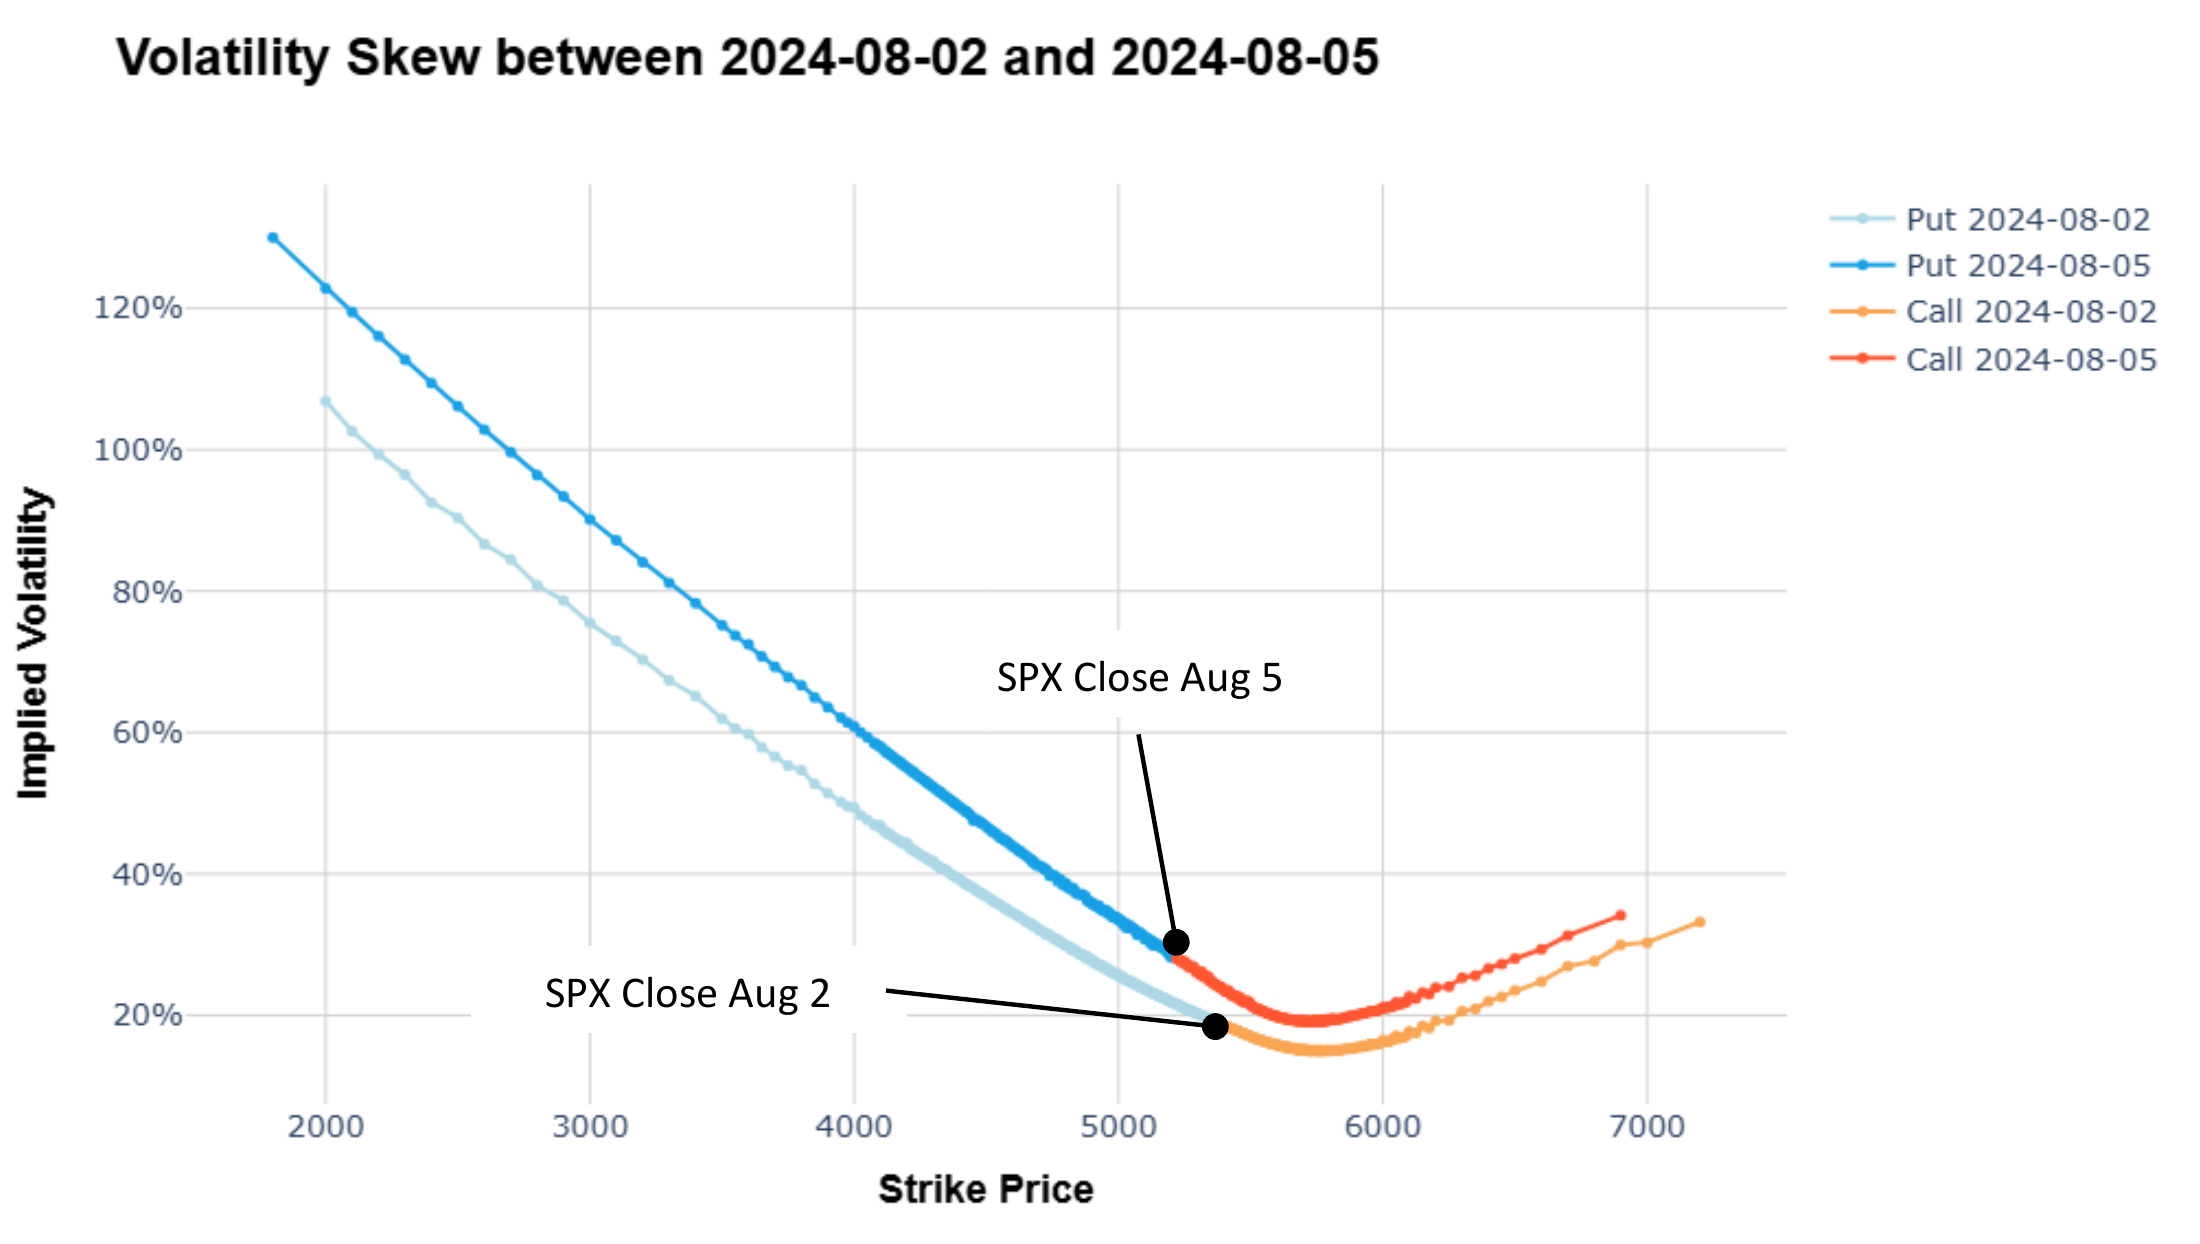
\includegraphics[width=0.72\textwidth]{../Figures/spx_skew_2024-08-02_2024-08-05.png}
\end{center}
\textbf{S\&P 500 options: downside skew.}
The two curves correspond to 2 and 5 August 2024, with a 30-day tenor
interpolated in variance between expiries. Near the money, lower strikes
carry higher implied volatilities. The right wing eventually rises too:
skew and smile curvature can coexist.

{\footnotesize Source: Cboe, Edward K.~Tom,
\href{https://cdn.cboe.com/resources/vix/VIX-Decomposition-2025-08-01.pdf}{\emph{The VIX Index Decomposition}},
1 August 2025, Exhibit 7, p.~9 (chart reproduced).
The chart legend and surrounding text date the observations to 2024;
the source's exhibit heading contains a year typo.\par}

\medskip
\begin{center}
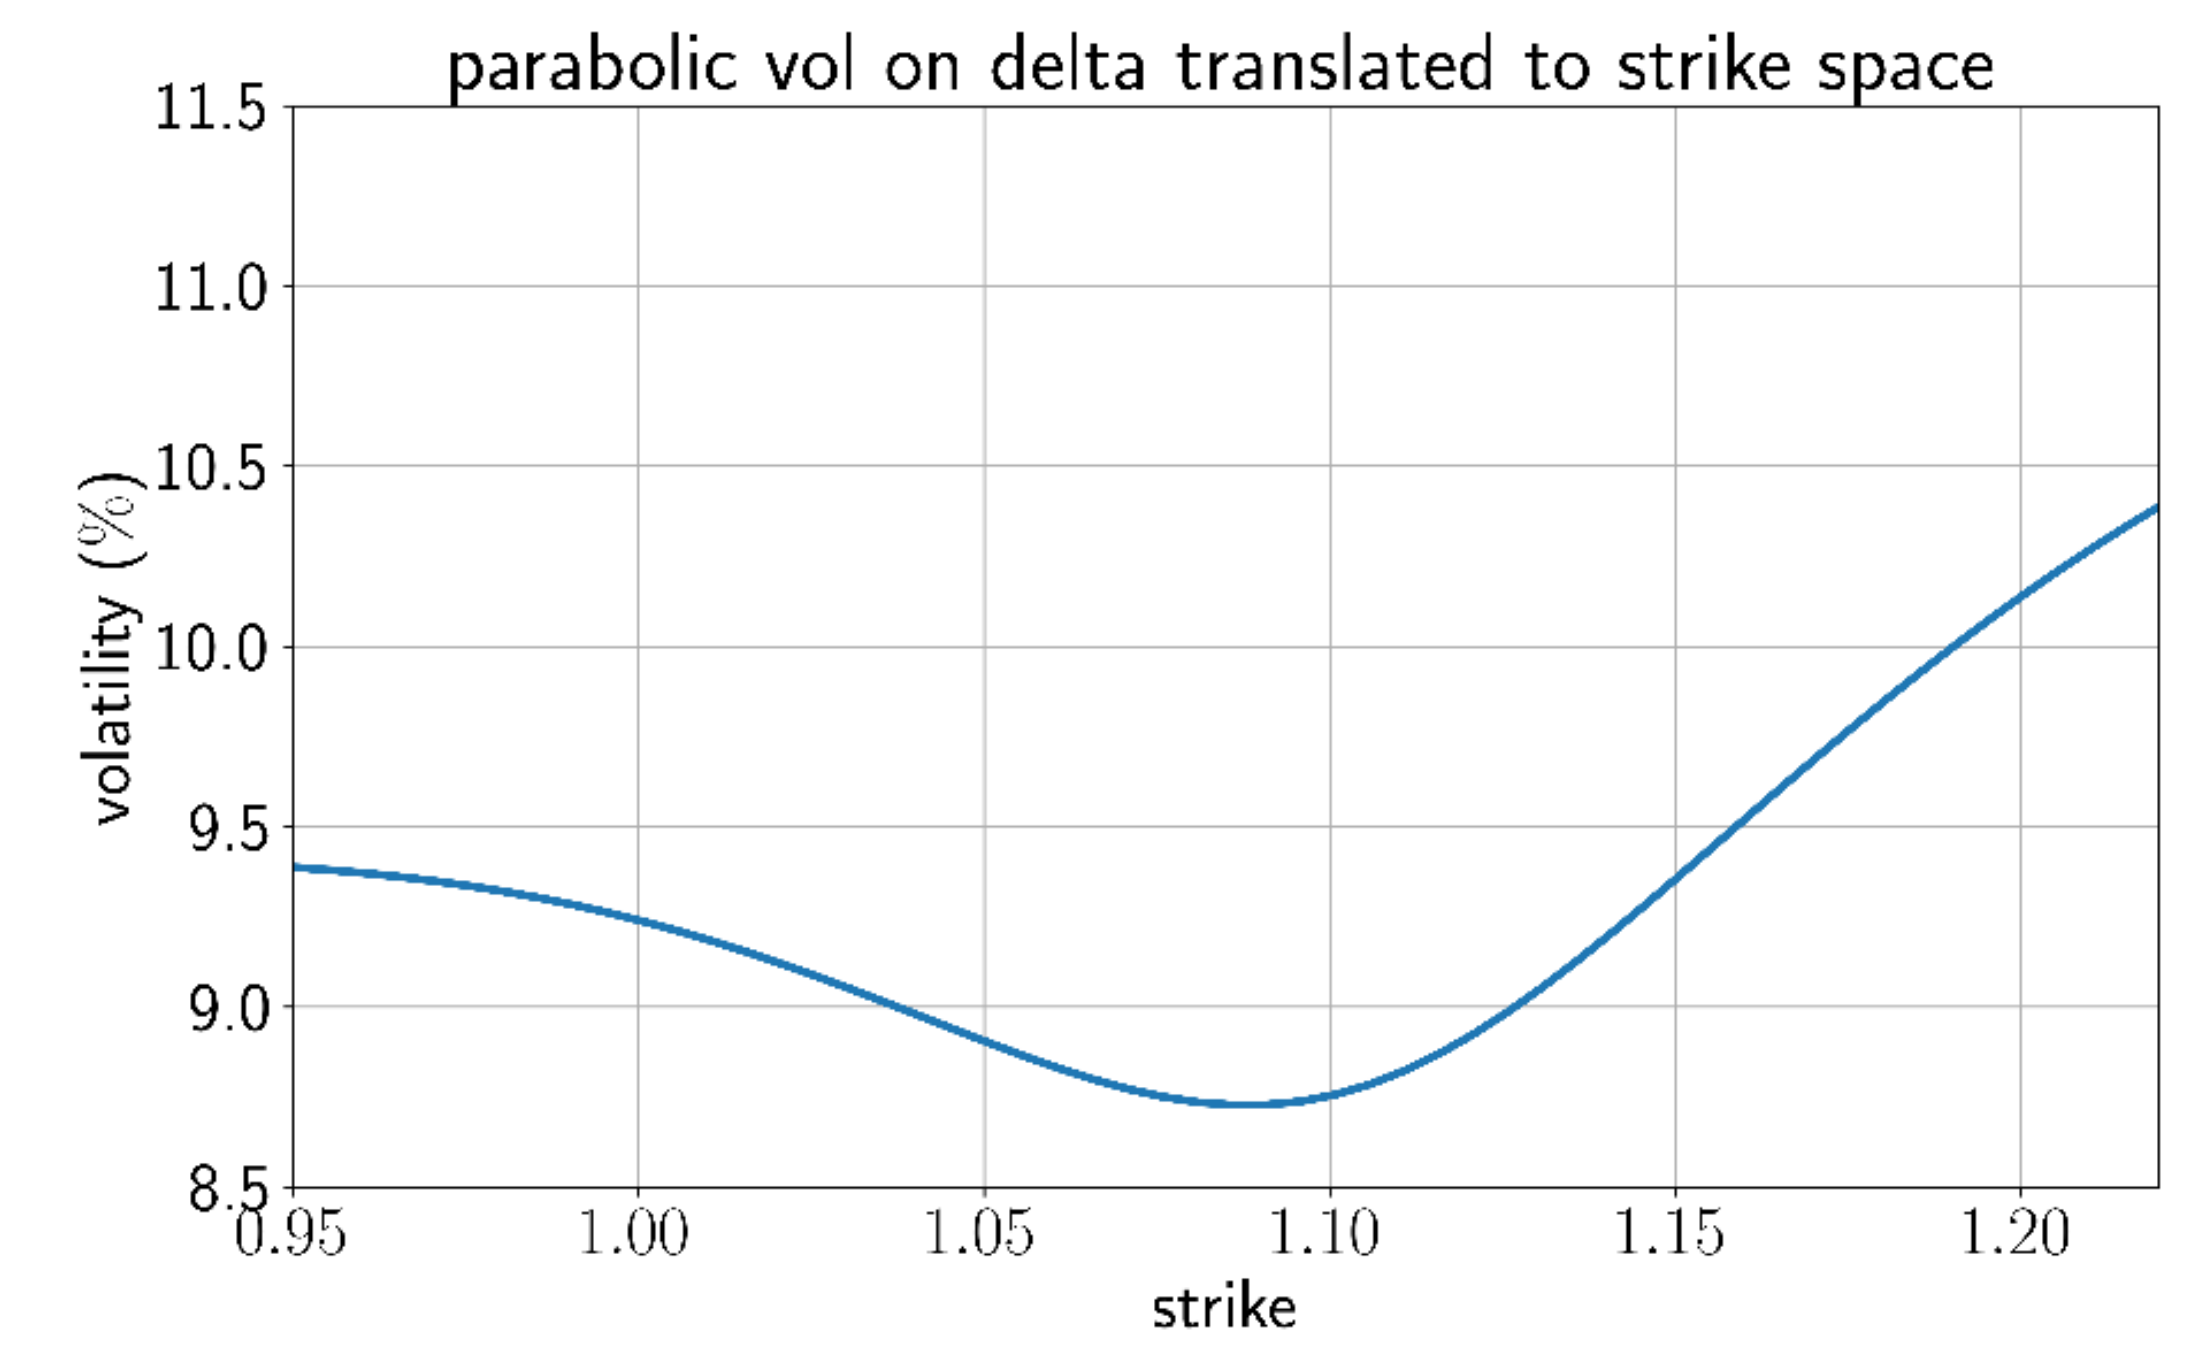
\includegraphics[width=0.66\textwidth]{../Figures/eurusd_smile_2025-04-23.png}
\end{center}
\textbf{EUR/USD options: an asymmetric smile.}
For a six-month tenor on 23 April 2025, both wings lie above the trough.
The strike is measured in USD per EUR. The smile is not symmetric, and
its minimum need not coincide with the spot or forward.

{\footnotesize Source: Uwe Wystup (MathFinance),
\href{https://www.mathfinance.com/wp-content/uploads/2025/06/FX-Column_2025-07_Why-digitals-dont-have-percentage-prices.pdf}{\emph{Why Digitals don't Have all Percentage Price Quotes}},
2025, Figure 2, p.~2; market quotes from ICE Data Services.
The author uses parabolic interpolation in delta, converts it to strike,
and fixes the reference spot at 1.1000 for illustration. This is a curve
constructed from market quotes, not a scatterplot of individual trades.\par}

\clearpage
% ============================================================
\section{Model-free bounds}
% ============================================================

\subsection{Calls and puts lie in known intervals}

\begin{proposition}[Basic no-arbitrage bounds]
With no dividends and \(D_t=e^{-r(T-t)}\),
\[
\boxed{\max(S_t-KD_t,0)\le C_t\le S_t,}
\qquad
\boxed{\max(KD_t-S_t,0)\le P_t\le KD_t.}
\]
\end{proposition}

\begin{proof}
For the call upper bound, one share superhedges the call because
\(S_T\ge(S_T-K)^+\). Thus a call cannot cost more than the share. If it did,
sell the call, buy the share, and retain the positive difference today.

For the lower bound, call positivity gives \(C_t\ge0\), and parity gives
\(C_t=P_t+S_t-KD_t\ge S_t-KD_t\) because \(P_t\ge0\). Combining them gives
the stated lower bound. The put bounds follow by the symmetric argument, or
by applying parity to the call bounds.
\end{proof}

\begin{studentexercise}{a fast quote check}
For \(S_t=K=100\), \(r=5\%\), and \(\tau=1\), classify call quotes \(2\),
\(10.45\), and \(103\) as impossible or potentially arbitrage-free.
\end{studentexercise}
\begin{shortsolution}
The bounds are
\[
\max(100-100e^{-0.05},0)\approx4.88\le C_t\le100.
\]
Thus \(2\) is too low, \(103\) is too high, and \(10.45\) is inside the
model-free interval. Being inside the interval is necessary, not sufficient,
for all cross-strike and cross-maturity consistency checks.
\end{shortsolution}

\subsection{Superhedges and subhedges}

The option bounds are instances of a general principle. If tradable portfolios
have terminal values \(Y_T\le H\le X_T\), their initial costs satisfy
\[
\boxed{Y_0\le\text{price}(H)\le X_0.}
\]
If the claim is more expensive than the superhedge, sell the claim and buy
the superhedge. If it is cheaper than the subhedge, buy the claim and short
the subhedge. In both cases the trade pays today and cannot lose at maturity.

% ============================================================
\section{Strike and maturity consistency}
% ============================================================

\subsection{Monotonicity in the strike}

\begin{proposition}[Strike monotonicity]
For the same underlying and maturity, if \(K_1<K_2\), then
\[
C_t(K_1)\ge C_t(K_2),
\qquad
P_t(K_1)\le P_t(K_2).
\]
\end{proposition}

\begin{proof}
For every terminal stock price,
\[
(S_T-K_1)^+\ge(S_T-K_2)^+.
\]
The lower-strike call dominates the higher-strike call, so it cannot be
cheaper. The put comparison reverses because the right to sell at a higher
price is more valuable.
\end{proof}

\begin{boardexample}{monotonicity arbitrage}
Suppose \(K_1=90<K_2=110\), but \(C_t(90)=8<C_t(110)=10\). Buy the
lower-strike call and sell the higher-strike call. The initial receipt is
\(2\), while the terminal payoff
\[
(S_T-90)^+-(S_T-110)^+\ge0
\]
in every state.
\end{boardexample}

\subsection{Convexity and butterfly spreads}

\begin{proposition}[Strike convexity]
For equally spaced strikes \(K-h<K<K+h\), an arbitrage-free call curve
satisfies
\[
\boxed{C_t(K-h)-2C_t(K)+C_t(K+h)\ge0.}
\]
Equivalently, \(K\mapsto C_t(K)\) is convex.
\end{proposition}

\begin{proof}
The butterfly payoff is
\[
(S_T-K+h)^+-2(S_T-K)^++(S_T-K-h)^+.
\]
It is zero outside \([K-h,K+h]\), increases linearly from zero to \(h\),
then decreases linearly to zero. It is therefore nonnegative in every state,
so its price must be nonnegative.
\end{proof}

\begin{studentexercise}{a butterfly quote check}
At equally spaced strikes \(90,100,110\), calls are quoted at
\(14,12,7\). Check monotonicity and convexity. If necessary, construct the
arbitrage.
\end{studentexercise}
\begin{shortsolution}
Monotonicity holds: \(14>12>7\). Convexity requires
\[
C_t(100)\le\tfrac12\big(C_t(90)+C_t(110)\big)=10.5,
\]
but the quote is \(12\). Buy the \(90\) and \(110\) calls and sell two
\(100\) calls. The initial cost is
\[
14+7-2(12)=-3,
\]
a receipt of \(3\), while the terminal butterfly payoff is nonnegative.
\end{shortsolution}

\subsection{A qualified maturity comparison}

If rates and dividends are zero and \(T_1<T_2\), calls with the same strike
satisfy
\[
C_t(K,T_2)\ge C_t(K,T_1).
\]
If this failed, buy the longer option and sell the shorter option. At
\(T_1\), the remaining longer option is worth at least the intrinsic value
needed to settle the short call. This is the calendar-spread argument.

\begin{warningbox}{Do not overstate calendar monotonicity}
Positive rates and dividends change the comparison across maturities. The
simple inequality above is a useful clean case, not a universal replacement
for the full calendar-arbitrage conditions used to construct option surfaces.
\end{warningbox}

% ============================================================
\section{Synthesis and practice}
% ============================================================

\begin{keyidea}{A practical order for quote diagnostics}
\begin{enumerate}
  \item Match the contract specifications: underlying, \(K\), \(T\), and dividends.
  \item Check positivity and the basic upper and lower bounds.
  \item Check put--call parity for calls and puts with the same \(K,T\).
  \item Across strikes, check monotonicity and convexity.
  \item Across maturities, use calendar checks with their stated assumptions.
  \item When an inequality fails, write the portfolio and its cashflows before
        labelling the opportunity an arbitrage.
\end{enumerate}
\end{keyidea}

\begin{studentexercise}{final diagnostic}
Assume no dividends. Given \(S_t=100\), \(K=100\), \(r=5\%\), \(\tau=1\),
\(C_t=12\), and \(P_t=5\), identify the inconsistency and construct the
trade.
\end{studentexercise}
\begin{shortsolution}
Since \(100e^{-0.05}=95.12\),
\[
C_t+KD_t=107.12>105=P_t+S_t.
\]
Sell the call, borrow \(95.12\), buy the put, and buy one share. The trade
receives \(2.12\) initially and has zero terminal net payoff by put--call
parity.
\end{shortsolution}

\begin{keyidea}{Final synthesis}
\[
\text{option payoff geometry}
\quad\Longrightarrow\quad
\text{arbitrage-free prices and hedges}.
\]
\end{keyidea}

\end{document}
